\documentclass[tikz,border=0mm]{standalone} 
\usetikzlibrary{positioning}
\usetikzlibrary{calc}
\usetikzlibrary{shadows.blur}
\usepackage{pgfplots}
%\usepgfplotslibrary{polar}
\pgfplotsset{compat=1.14}
\usepackage{ifthen}
\usepackage{amsmath}
\newcommand{\dirlabel}[1]{
	\scalebox{0.8}{\scriptsize\textsf{\textcolor{black}{#1}}}
}
\begin{document}
\fontfamily{phv}\selectfont
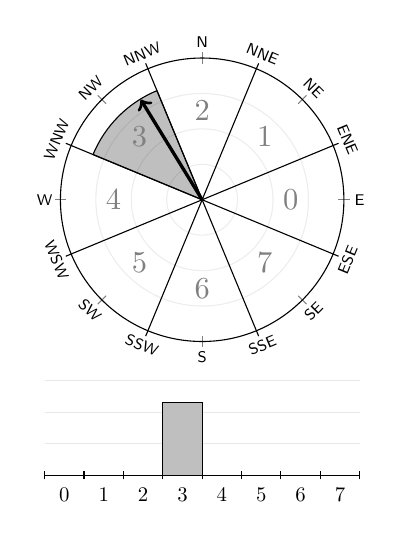
\begin{tikzpicture}


\draw[draw=black, fill=black!25] (0,0) --  (112.5:1.5) arc(112.5:157.5:1.5) -- cycle;

\foreach \a in {0,...,7} {
	\draw[gray]  ({(\a+0.0)*45}:1.725) -- ({(\a+0.0)*45}:1.875);
	\draw[black] (0,0) -- ({(\a+0.5)*45}:1.875);
	\draw node at ({(\a+0.0)*45}:1.125) {\scalebox{1.1}{\textcolor{black!50}{\a}}};
}
\draw (0,0) circle (1.8cm);

\node[rotate=0] at(0:2) {\dirlabel{E}};
\node[rotate=-67.5] at(22.5:2) {\dirlabel{ENE}};
\node[rotate=-45] at(45:2) {\dirlabel{NE}};
\node[rotate=-22.5] at(67.5:2) {\dirlabel{NNE}};
\node[rotate=0] at(90:2) {\dirlabel{N}};
\node[rotate=22.5] at(112.5:2) {\dirlabel{NNW}};
\node[rotate=45] at(135:2) {\dirlabel{NW}};
\node[rotate=67.5] at(157.5:2) {\dirlabel{WNW}};
\node[rotate=0] at(180:2) {\dirlabel{W}};
\node[rotate=-67.5] at(-157.5:2) {\dirlabel{WSW}};
\node[rotate=-45] at(-135.5:2) {\dirlabel{SW}};
\node[rotate=-22.5] at(-112.5:2) {\dirlabel{SSW}};
\node[rotate=0] at(-90:2) {\dirlabel{S}};
\node[rotate=22.5] at(-67.5:2) {\dirlabel{SSE}};
\node[rotate=45] at(-45:2) {\dirlabel{SE}};
\node[rotate=67.5] at(-22.5:2) {\dirlabel{ESE}};

\draw[->, very thick] (0,0) -- (121.5:1.49);


\begin{scope}[xshift=-2cm, yshift=-3.5cm]
\draw (0cm, 0cm) -- (4cm, 0cm);
\foreach \h in {1,...,3}
	\draw[black!9!white] (0cm, 0.4*\h cm) -- (4cm, 0.4*\h cm);
\draw[fill=black!25] (1.5cm, 0cm) -- (1.5cm, 0.93cm) -- (2cm,0.93cm) -- (2cm,0cm) -- cycle;
\foreach \a in {0,...,7}
	\node at (0.5*\a cm +0.25 cm, -0.25cm) {\scalebox{0.75}{\a}};
\foreach \a in {0,...,8}
	\draw (0.5*\a cm, -0.05cm) -- (0.5*\a cm, 0.05cm);
\end{scope}

\draw[opacity=0.07] (0,0) circle (0.45cm);
\draw[opacity=0.07] (0,0) circle (0.9cm);
\draw[opacity=0.07] (0,0) circle (1.35cm);
\end{tikzpicture}
\end{document}